\documentclass[14pt]{extarticle}
\usepackage[
left=30mm,
top=20mm,
right=15mm,
bottom=20mm,
]{geometry}

\usepackage{graphicx}
\usepackage[utf8x]{inputenc}
\usepackage[russian]{babel}
\usepackage[T1]{fontenc}
\usepackage{float}
\usepackage{listings}
\usepackage{cite}
\usepackage{hyperref}
\usepackage{etoolbox}
\usepackage{indentfirst}
\usepackage[linesnumbered,boxed]{algorithm2e}
\sloppy

\graphicspath{{Figures//}}%путь к рисункам


\lstset{inputencoding=utf8x, extendedchars=false, keepspaces = true,
language=C++,
keywords={include, const, virtual, template, typename, class, private, public, operator, if, while, else, return, new, delete, int, float, bool, char},
sensitive=true,
%basicstyle=\small,
commentstyle=\scriptsize\rmfamily,
keywordstyle=\ttfamily\underbar,
identifierstyle=\ttfamily,
basewidth={0.5em,0.5em},
columns=fixed,
fontadjust=true,
breaklines=true,
literate={->}{{$\to$}}1
}

\makeatletter
\renewcommand{\@biblabel}[1]{#1.} % Заменяем библиографию с квадратных скобок на точку:
\makeatother
\gappto\captionsrussian{\renewcommand{\contentsname}{Оглавление}}
\renewcommand\baselinestretch{1.5}
\renewcommand{\lstlistingname}{Результат}

\begin{document}

\begin{titlepage}
\thispagestyle{empty}
\def\baselinestretch{1.0}
\begin{center}
	{САНКТ-ПЕТЕРБУРГСКИЙ ГОСУДАРСТВЕННЫЙ УНИВЕРСИТЕТ \\ \vskip 0.3em {\large Математико-механический факультет \\ \vskip 0.7em{\large Кафедра информатики \\}}}
    \vspace*{0.15\textheight}
    {\large Крень Мария}
    
    \vskip 2em
    {\huge Пользовательский уровень библиотеки неконсервативной сборки мусора для C++}
    
    \vskip 1em
    {\large Дипломная работа} \\
    \vskip 2em
    {\normalsize \raggedleft 
    Допущена к защите.\\
    Зав. кафедрой:\\
    д.ф.-м.н., Н.К.Косовский 
    \\[3em]
    Научный руководитель:\\
    к.ф.-м.н. Д.Ю.Булычев
    \\[3em]
    Рецензент:\\
    к.ф.-м.н. Д.В.Кознов\\
    \vspace*{0.08\textheight}
    {\centering Санкт-Петербург \\ 2014}
    }
\end{center}
\end{titlepage}
\begin{titlepage}
\thispagestyle{empty}
\def\baselinestretch{1.0}
\begin{center}
	{\large SAINT-PETERSBURG STATE UNIVERSITY \\ \vskip 0.3em {\large Mathematics and Mechanics Faculty \\ \vskip 0.7em{\large Informatics Chair \\}}}
    \vspace*{0.15\textheight}
    {\large Mariya Kren}
    
    \vskip 2em
    {\huge User Level of a Non-Conservative Garbage Collection Library for C++}
    
    \vskip 1em
    {\large Graduation Thesis} \\
    \vskip 2em
    {\normalsize \raggedleft 
    Admitted for defence.\\
    Head of the chair:\\
    professor N.K. Kosovsky
    \\[3em]
    Scientific supervisor:\\
    Dr. D.Yu. Boulytchev
    \\[3em]
    Reviewer:\\
    Dr. D.V.Koznov\\
    \vspace*{0.08\textheight}
    {\centering Saint-Petersburg \\ 2014}
    }
\end{center}
\end{titlepage}
\tableofcontents
\thispagestyle{empty} 
\setcounter{page}{4}
\section*{Введение}
\addcontentsline{toc}{section}{Введение}
Программисту важно писать  код свободный от ошибок. Наиболее уязвимым местом в коде с точки зрения человеческого фактора является ручное управление динамической памятью.  Безопасное управление памятью значительно повышает надёжность программной системы, исключая многие распространённые ошибки, которые могут возникать из-за обычной опечатки и требовать длительного поиска, а зачастую  -  оставаться вообще неисправленными. Поэтому в любом современном языке программирования и окружающем его инструментарии используется технология сборки мусора. Почему сборка мусора? Потому что, этот механизм обладает рядом важных преимуществ над ручным управлением памяти, одно из которых -- безопасноть. Под безопасным управлением памятью подразумеваются средства языка программирования и его системы времени выполнения, которые гарантируют защиту от ошибок при работе с динамической памятью.
 
Сборка мусора — это один из споcобов автоматического управления динамической памятью. Суть сборки мусора заключается в том, что выделенная в приложении память, которая ему в дальнейшем не понадобится, освобождается системой управления памятью автоматически. Для этого в определённые моменты запускается процесс, называемый сборкой мусора.
 
Сборка мусора обладает как достоинствами, так и недостатками. По сравнению с ручным управлением, автоматическое управление памятью безопаснее: программисту не нужно заботиться о том, когда освобождать память из-под объектов. Это дает гарантию того, что не возникнет некоторых ошибок, таких как: висячий указатель, т.е. указатель на уже освобожденный объект, или ошибка повторного освобождения памяти, когда программа пытается освободить память, которая уже была освобождена.

С другой стороны при автоматическом управлении памятью могут возникнуть следующие проблемы:
\begin{enumerate}
\item Если на объект есть ссылки из других достижимых объектов, то он никогда не будет удален.
\item Во время работы программы из-за прогресса сборщика мусора возникают паузы в случайные моменты времени, а их продолжительность не определена.
\item  Должны быть выполнены требования для реализации сборщика мусора.
\end{enumerate}
Во-первых, должна присутствовать возможность определить все указатели из любого объекта на другие элементы кучи.
Во-вторых, не должно быть никаких операций над указателями (логических, арифметических и т.п.)
Помимо этого, приходится затрачивать время на отслеживание дополнительной информации по объектам.


\pagebreak

Помимо этого, приходится затрачивать время на отслеживание дополнительной информации по объектам.
 
Впервые сборка мусора была применена еще  в 1959 году Джоном Маккартни. Он использовал ее в среде программирования для разработанного им языка функционального программирования Lisp. В дальнейшем сборку мусора стали применять преимущественно в функциональных и логических языках. Необходимость сборки мусора в языках этих типов обусловлена тем, что структура таких языков делает крайне неудобным отслеживание времени жизни объектов в памяти и ручное управление ею .
 
В промышленных процедурных и объектно-ориентированных языках технология сборки мусора стала приобретать популярность лишь со второй половины 1980-х годов. До этого времени ручное управление памятью считалось предпочтительнее, как более эффективное и безопасное. Со второй половины 1990-х годов все чаще и чаще механизм сборки мусора включали в языки и среды, ориентированные на прикладное программирование. После появляния языка программирования Java в 1995 году, сборка мусора стала настоящим “мейнстримом”.  На данный момент, технология сборки мусора используется в таких языках, как Java, C\#, Python, Ruby, Perl и т.д.
Язык С++ является одним из самых сложных языков программирования. Свою популярность он приобрел благодаря своей гибкости, пригодности для программирования шикрокого класса задач. Несмотря на то , что язык С++ появился более 30 лет назад, до сих пор в нем не существует стандартных  технологий сборки мусора. По этой причине программисты используют  малоэффективные средства автоматического управления динамической памятью, такие как смартпойнтеры, счетчики ссылок, пулы и прочие .

Данная дипломная работа посвящена вопросу о том, как организовать сборку мусора для С++ так, чтобы она была неконсервативной (точной) и  поддерживала языковые примитивы C++.
\newpage
\section{Постановка задачи}
Целью данной работы является создание пользовательского уровня для неконсервативного сборщика мусора для С++, реализованного в рамках проекта jbgc [куча ссылок на статьи с описанием + сноска на проект на гитхабе].


\vspace{0.3cm}
 Следующие основные подзадачи были выделены для её достижения:
\begin{itemize}
\item Изучить и проанализировать существующие подходы к неконсервативной сборке мусора и их реализацию на пользовательском уровне в разных языках, оценить их применимость для языка С++;
\item Предложить и реализовать собственное решение на основе проведенного анализа в связи с отсутствием сборщиков мусора для С++;
\item Продемонстрировать работоспособность реализованного сборщика мусора на пользовательском уровне;

\end{itemize}
\newpage
\section{Некоторые средства автоматизации\\
управления памятью для С++}

Одним из наиболее широко используемых средств автоматизации управления памятью в
контексте языка С++ являются ``умные указатели'' (smart pointers). ``Умный указатель''~---
это специальный объект, который хранит указатель на участок динамически отведенной области
памяти и определяет некоторую дисциплину обращения с этом указателем. Иногда следование
этой дисциплине является лишь соглашением, и тогда ``умный указатель'' является всего лишь
способом идентифицировать необходимость правильного обращения с данными; однако довольно часто
``умные указатели'' действительно определенным образом ограничивают набор возможных
способов манипулирования данными за счет использования декларативных возможностей языка С++.

Простейший ``умный указатель'' может выглядеть так:

\begin{lstlisting}
    template <typename T> class smart_pointer {
      T *m_obj; // Указатель на динамические данные
      public:
        // Конструктор получает исходный указатель 
        smart_pointer (T *obj) : m_obj(obj) {}
        // Деструктор удаляет адресуемые данные
        ~smart_pointer () { delete m_obj; }
        // Перегруженные операторы для обращения к данным
        T* operator-> () { return m_obj; }
        T& operator*  () { return *m_obj; }
    }
\end{lstlisting}

Такой указатель позволяет обеспечить автоматическое освобождение области динамической памяти, если 
время её жизни можно ограничить временем жизни самого ``умного указателя''. При этом никак не
контролируется, что сам ``умный указатель'' используется правильно --- например, что конструктор
получает действительно адрес в куче или что для данного адреса создан только один ``умный указатель''.

Другим примером ``умного указателя''является \lstinline{Boost::scoped_ptr}\footnote{\url{http://www.boost.org/doc/libs/1_39_0/libs/smart_ptr/scoped_ptr.htm}} 
библиотеки BOOST\footnote{\url{http://www.boost.org}}. Его основное отличие от приведенного выше~--- отсутствие возможности копирования и присваивания (а,
значит, и передачи параметром в функцию). Эти ограничения не исключают возможность неправильного использования, но позволяют избежать некоторых из них.

Еще одним вариантом является \lstinline{auto_ptr}\footnote{\url{http://www.cplusplus.com/reference/memory/auto_ptr}}. Этот указатель разрешает
операции копирования и передачи параметром, но при этом ``опустошается'' содержимое источника. Таким образом, указатели не копируются, 
а ``перемещаются'', что позволяет избежать ситуации, когда происходит несколько попыток освободить одну и ту же область памяти из-за хранения 
её адреса разными ``умными указателями''. С другой стороны, теперь не гарантируется, что ``умный указатель'' всегда указывает на правильные данные ---
в какой-то момент он может ``испортиться''. В силу этого такие указатели нельзя использовать в контейнерах STL. Для таких целей используются
\lstinline{std::shared_ptr}.

\lstinline{shared_ptr}\footnote{\url{http://www.cplusplus.com/reference/memory/shared_ptr}}~--- это ``умный указатель'' с подсчетом ссылок. Это значит, 
что с каждой областью памяти, адресуемой \lstinline{shared_ptr}, ассоциирована переменная, которая хранит количество указателей, которые ссылаются на начало
этой области памяти. Если эта переменная становится равной нулю, то область освобождается. Счетчик инкрементируется при каждом вызове оператора копирования 
или оператора присваивания. У \lstinline{shared_ptr} есть оператор приведения к типу \lstinline{bool}, что позволяет проверять, указывает ли он на что-нибудь.
Использование \lstinline{shared_ptr} может обеспечить сравнительно безопасную автоматизацию управления памятью, однако неприятности все же возможны. Во-первых,
наличие указателя \lstinline{shared_ptr} не на начало динамически отведенной области памяти не гарантирует её сохранения; кроме того, циклические
ссылки приводят к образованию неудаляемого мусора; наконец, возможна ситуация лавинообразного освобождения памяти с возникновением непредсказуемой
задержки.

\newpage
\section{Особенности языка С++}

 
Во введении мы выяснили, что “С++” - сложный язык программирования широкого назначения. На этом языке написано огромное количество всевозможных продуктов, таких как операционные системы, разнообразные прикладные программы, драйверы устройств, приложения для встраиваемых систем, высокопроизводительные серверы, а также развлекательные приложения.
Однако, у “С++” есть один крупный недостаток. Заключается он в том, что данный язык, в отличии от таких языков как Java, не предназначен для “сборки мусора”, вследствие чего под угрозу ставится производительность и безопасность кода.

\subsection{Введение} 

Как уже было сказано ранее, язык С++, изначально не предназначен для сборки мусора. Но с новыми стандартами язык становится более простым и удобным в использовании, появляются новые инструменты, операторы. Это позволяет подумать над тем, как организовать процесс сборки мусора так, чтобы программы удовлетворяющие ряду ограничений могли запускать этот процесс.

При реализации сборщика мусора JBGC был использован ряд новшевств, вошедших в последний стандарт языка С++ -- С++11, а также некоторые инструменты и операторы, описанные еще в более поздних стандартах: 
\begin{enumerate}
\item оператор typeid;
\item шаблоны простые и с переменным числом аргументов -  template ,variadic template;
\item  конструкторы, деструкторы и порядок их вызова;
\end{enumerate}
Далее рассмотрим вышеперечисленные пункты подробнее.
\subsection{Оператор typeid} 

В реализации сборщика мусора JBGC для осуществления обхода и маркировки всех объектов хранится метаинфомация.  Метаинформация создается не для каждого объекта, а для конкретного типа. Этого оказалось достаточно, для того, чтобы получить необходимую для сборщики мусора информацию. Набор всех указателей на метаинформацию хранится в отдельном списке. По типу объекта можно получить указатель на метаинформацию соответствующую типу с помощью специальной функции.

Каждый раз, при вызове gc\_new, для объекта происходит проверка на существование метаинформации для заданного типа объекта. Если метаинформация лежит в списке, то возвращатся указатель на нее и кладется в начало объекта, если нет, то конструируется новая, и указатель на метаинформацию добавляется в  специальный список с типом-ключом.

Для того, чтобы такой подход стал возможным, нужен инструмент, который позволит идентифицировать тип во время исполнения(run-time type identification -- RTTI\footnote{ http://msdn.microsoft.com/en-us/library/b2ay8610.aspx}). Такая возможность существует в языке С++ -- функция \textit{typeid}. Для использования этой функции необходимо включить заголовочный файл typeinfo.h, а также установить режим поддержки RTTI в опциях компилятора. Форма записи данно функции имеет следующий вид:
\lstinline[language= C++]{typeid(object)}, где object -- объект, чей тип следует определить. Функция \textit{typeid} вернет ссылку на объект типа typeinfo, который описывает тип объекта object. 

Когда функция \textit{typeid} применяется к указателю на базовый класс полиморфного класса, она автоматически возвращает тип объекта, на который указывает указатель, в том числе любой класс, выведенный из базового класса. (Как уже говорилось, полиморфным классом называется класс, содержащий хотя бы одну виртуальную функцию.)\footnote{http://www.c-cpp.ru/books/identifikaciya-tipa-vo-vremya-ispolneniya-rtti}

Следующий кусок кода gc\_new JBGC демонстрирует использование функции \textit{typeid}:
\begin{lstlisting}[language= C++]

/* если количество смещений внутри объекта равно нулю */
if (sizeOfPointerList(offsets) == 0) { 
	if (DEBUGE_MODE) {
		printf("if (offsets.size() == 0) {\n");
		fflush(stdout);
	}
	/* если в списке пар содержится данная пара */
	if (contains(classMeta, typeid(T).name())) { 
		if (DEBUGE_MODE) {
			printf("contains meta for class %s\n", typeid(T).name());
		}
		/* получить указатель на метаинформацию для данной пары */
		m_inf->shell = getClassMetaPointer(classMeta, typeid(T).name());  
	}
	/* если в списке пар соответствий не найдено */ 
	else {
		 if (DEBUGE_MODE) {
			 printf("new meta for class %s\n", typeid(T).name());
 	}
	/* создать новую метаинформацию, вернуть указатель на нее,
	      записать в начало объекта */
	 m_inf->shell = generic_box_simple ();
	/* добавить новую пару в список */
	 addNewClassMetaInformation(typeid(T).name(), m_inf->shell); 
     }
\end{lstlisting}


\subsection{Template, variadic template} 

В сборщике мусора JBGC функция выделения памяти для шаблонов-объектов (англ.template objects) gc\_new  использует оператор \textit{placement new} (производит размещение (инициализацию) объекта путем вызова конструктора, и создание в памяти по указанному адресу\footnote{http://www.cplusplus.com/reference/new}) для инициализации классом области памяти. Для вызова в подобном случае конструктора не по умолчанию у шаблона-объекта,  используется шаблон с переменным числом аргументов (англ. varidic templates), предоставляющий информацию о типах передаваемых объектов.

\textit{Шаблоны} (англ. template) — средство языка C++, предназначенное для кодирования обобщённых алгоритмов, без привязки к некоторым параметрам (например, типам данных, размерам буферов, значениям по умолчанию). 

\textit{Шаблон с переменным числом аргументов}(англ. variadic template) — это класс или шаблон функции, поддерживающий произвольное число аргументов. Этот механизм особенно удобен для разработчиков библиотек C++, поскольку можно применить его к обоим шаблонам класса и шаблоны функций и таким образом предоставляют широкий спектр типобезопасных и нетривиальных функции и гибкости. Возможность использовать шаблоны с переменным числом аргументов появилась только в новом стандарте С++ -- С++11. 

Рассмотрим пример использования сборщика мусора JBGC  с конструктором объекта не по умолчанию,  наглядно демонстрирующий необходимость использования шаблона с переменным числом аргументов:

\begin{lstlisting}[language= C++]
#include <libgc/libgc.h>
#include <stdio.h>

class A {
private:
	int size;
	gc_ptr<int> mas;
public:
  	// A () {}

	/* конструктор не по умолчанию*/
	A (int len, const gc_ptr<int> & ar) {
		printf("A ... ");
		fflush(stdout);
		size = len;
		this->mas = gc_new<int>(len);
		printf("gc_new...ends\n");
		fflush(stdout);
		for (int i = 0; i < len; i++) {
			mas[i] = ar[i];
		}
	printf("ends\n");
	fflush(stdout);
  	}
};

int main (void) {
	int len = 10;
	/* создается два умных указателя, первый на массив int, длины len ,второй такой же */
	gc_ptr<int> ar = gc_new<int>(len), br = gc_new<int>(len);
	
	/* заполняются массивы */
	for (int i = 0; i < len; i++) {
		ar[i] = i;
		 br[i] = len - i;
	}
	/* создается умный указатель на объект класса А */
	/* у умного указателя аргументы: имя класса, имя типа первого,второго поля;
	    * в круглых скобках  имена передаваемых конструктору объектов
	    */
	/* здесь и нужен шаблон с переменным числом аргументов,
	    * иначе не понятно, как определить тип второго объекта в конструкторе 
	    */
	gc_ptr<A> a = gc_new<A, int, gc_ptr<int>&>(len, ar);
	gc_ptr<A> b = gc_new<A, int, gc_ptr<int>&>(len, br);
	for (int i = 0; i < len; i++) {
		ar[i] += 10;
		br[i] += 100;
  	}
	a->print(); b->print();
	printf("\n");
	return 0;
}

\end{lstlisting}
 \subsection{Конструкторы, деструкторы и порядок их вызова} 

Важным фактом является то, что в С++  момент создания/удаления объекта можно отследить с помощью \textit{конструктора/деструктора} объекта. В сборщике мусора JBGC этот факт является одним из основопологающих всего процесса. При вызове конструктора gc\_ptr , вызывается функция добавления себя в список корней, в случае загрузки стековой рамки на стек и функцию удаления себя из этого списка в своем деструкторе, в случае вытеснения стековой рамки. Заметим, что порядок вызова деструкторов противоположен порядку вызову конструкторов. 
\newpage
\section {Пользовательский уровень сборщика мусора JBGC}

\subsection {Использование JBGC}
Для того, чтобы воспользоваться сборщиком мусора JBGC нужно сначала установить его на ваш компьютер. Сборщик мусора изначально написан под Ubuntu. Работает он в системах семейства Linux. Для того, чтобы его установить, нужно выполнить последовательно следующие команды в терминале:
\begin{enumerate}
\item ./autogen.sh
\item ./configure
\item make clean | make | make install
\end {enumerate}

При запуске программы обязательно указывать переменную окружения LD\_LIBRARY\_PATH \footnote{URL: \url{http://www.opennet.ru/base/dev}}, список отделённых  двоеточиями  имён каталогов, где библиотеку JBGC -- gc следует искать перед  тем,  как  их  будут  искать  по стандартным путям.

Программа, использующая сборщик мусора JBGC должна удовлетворять следующим ограничениям:
\begin{enumerate}
\item Все указатели  должны быть заменены на  объекты класса gc\_ptr -- gc\_ptr<typename> \begin{lstlisting}int* a; ->  gc_ptr<int> a;
\end{lstlisting}
\item Все вызовы new заменены на gc\_new<typenames>(params)(size\_t size) \begin{lstlisting} new int [5]; -> gc_new<int>(5);
\end{lstlisting}
\end {enumerate}
А также нужно сделать include заголовочного файла:\begin{lstlisting}
#include <libgc/libgc.h>;
\end{lstlisting}

Небольшая программка, использующая сборщик мусора JBGC:
\begin{lstlisting}
#include <cstdio>
#include <libgc/libgc.h>

class point {
	int x,y
}

int main() {
	gc_ptr<point> pt;
	gc_ptr<int> p;

	pt = gc_new<point>();
	p = gc_new<int>();
}

\end{lstlisting}
\subsection {Возможности ``умного указателя'' gc\_ptr}
В следствие одного из главных требований, накладываемых на реализацию сборщика мусора:  не должно быть никаких операций над указателями (логических, арифметических и т.п.), был реализован набор операторов для работы с gc\_ptr:

\begin{enumerate}
\item (*) или разыменовывания -- примененная к gc\_ptr, обеспечивает доступ к содержимому ячейки памяти, на которую ссылается указатель. 
Пример использования:
\begin{lstlisting}
int a = 5, b = 6;
gc_ptr<int> ar = &a, br = &b;
* ar = 10;
* br = *ar;
\end{lstlisting}

\item  (->) или стрелка, обеспечивает доступ к элементам структур.

Пример:
\begin{lstlisting}
struct A {
	int a;
	int b;
}
/* создается gc_ptr на структуру A */
gc_ptr<A> obj = gc_new<A>();
/* обращение к полям структуры */
obj -> a = 5;
obj -> b = 6;
\end{lstlisting}

\item ([ ]) или обращения к элементу. 

Пример:
\begin{lstlisting}
/* создается массив элементов типа int длины len */
gc_ptr<int> ar = gc_new<int>(len), br = gc_new<int>(len);
	for (int i = 0; i < len; i++) {
		ar[i] = i;
		br[i] = len - i;
	}
\end{lstlisting}

\item (==) или проверки на равенство, вернет соответственно true и false, только если gc\_ptr указывают на один и тот же объект. 

Пример:
\begin{lstlisting}
int a = 5, b = 6;
int * ar2 = &a, br2 = &b;
gc_ptr<int> ar = &a, br = &b;
/* в этом случае результат будет false */
if (ar == br) {
...	
}
/* в этом случае результат будет true */
if (ar== ar2) {
...
}

/* в этом случае результат будет false */
if (ar == 0) {
...
}
\end{lstlisting}

\item (!=) или проверки на неравенство, вернет соответственно true и false, только если gc\_ptr указывают на разные объекты. 

Пример:
\begin{lstlisting}
int a = 5, b = 6;
int * ar2 = &a, br2 = &b;
с
/* результат будет true */
if (ar != br) {
...	
}
/* результат будет false */
if (ar != ar2) {
...
}
if (ar !=  0) {
...
}
\end{lstlisting}

\item (=) или присваивания. 

Пример:
\begin{lstlisting}
int a = 5;
int * ar2 = &a;
gc_ptr<int> ar = gc_new<int>();
gc_ptr<int> br = gc_new<int>();
ar = ar2;
br = ar;
\end{lstlisting}

\end {enumerate}

Представленных операций достаточно для того, чтобы реализовать основные примитивы языка С++.

\subsection{ Возможности функции выделения памяти gc\_new}

В языке С++ существует пять различных вариантов вызова функции выделения памяти для объекта --- new. Оператор пытается выделить достаточно памяти в куче для размещения новых данных и, в случае успеха, возвращает адрес свежевыделенной памяти. После выделения памяти вызывается конструктор объекта. Однако, если new не может выделить память в куче, то он передаст (throw) исключение типа std::bad\_alloc. Это устраняет необходимость явной проверки результата выделения. После встречи компилятором ключевого слова new им генерируется вызов конструктора класса.
\begin {enumerate}

\item \textit{new type} -- выделение памяти под обект типа type, кроме объектов структур, классов. 

Пример:
 \begin{lstlisting}
float* pf = new float;
\end{lstlisting}
 
\item \textit{new A()} -- выделение памяти под объект класса/структуры, после этого вызов конструктора по умолчанию. 

Пример:
 \begin{lstlisting}
class CName {
public:
   enum {
      sizeOfBuffer = 256
   };

};
int main() {
   CName* pName = new CName;
}
\end{lstlisting}

\item\textit{ new type [len]} -- выделение памяти под массив, состоящий из элементов типа type, длинной len.

 Пример:
 \begin{lstlisting}
  int* p_array = new int[5];
\end{lstlisting}

\item \textit{new A(p1, p2, ...)} -- выделение памяти под объект класса A, после этого вызов конструктора не по умолчанию. 

Пример:
 \begin{lstlisting}
class A {
private:
	int size;
	int * mas;
public:
	A () {}
	~A () {}

	A (int len, const int * & ar) {
		size = len;
		this -> mas =new  int [len];
		for (int i = 0; i < len; i++) {
			mas[i] = ar[i];
		}
	}
	};
int main () {
	A* a = new A (len, ar);
	A* b = new A (len, br);
	for (int i = 0; i < len; i++) {
		ar[i] += 10;
		br[i] += 100;
	}
	return 0;
}
\end{lstlisting}
\end {enumerate}

Для gc\_new существуют вызовы по-сути схожие стандартным вызовам new.
\begin {enumerate}
\item \textit{gc\_new<type>()} --  выделение памяти под обект типа type, кроме структур, классов. 
Пример:
 \begin{lstlisting}
gc_ptr<float> pf = gc_new <float>();
\end{lstlisting}
\item \textit{gc\_new< class\_name>()} -- выделение памяти под объект класса/структуры, после вызов конструктора по умолчанию. 
Пример:
 \begin{lstlisting}
class CName {
public:
   enum {
      sizeOfBuffer = 256
   };

};
int main() {
  gc_ptr<CName> pName = gc_new< CName>();
}
\end{lstlisting}

\item \textit{gc\_new <type>(len)} -- выделение памяти под массив из элементов типа type, c количеством элементов len. 
Пример:
 \begin{lstlisting}
 gc_ptr<int> p_array = gc_new <int>(5);
\end{lstlisting}

\item \textit{gc\_new <class\_name, types\_of\_objects...>(список аргументов конструктора не по умолчанию)} -- выделение памяти под обект класса/структуры. В треугольных скобках слева направо аргументы: class\_name -- имя класса/структуры объекта, под который отводится память; types\_of\_objects -- список типов объектов, присутствующих в конструкторе, строго в порядке указания в конструкторе; список имен объектов или значений, передаваемых конструктору(список аргументов в круглых скобках). 
Пример:
 \begin{lstlisting}
class A {
private:
	int size;
	gc_ptr<int> mas;
public:
	A () {}
	~A () {}

	A (int len, const gc_ptr<int> & ar) {
		size = len;
		this -> mas = gc_new<int>(len);
		for (int i = 0; i < len; i++) {
			mas[i] = ar[i];
		}
	}
};
int main () {
	gc_ptr<A> a = gc_new<A, int, gc_ptr<int>&>(len, ar);
	gc_ptr<A> b = gc_new<A, int, gc_ptr<int>&>(len, br);
	return 0;
}
\end{lstlisting}
\end {enumerate}

Таким образом процесс выделения памяти в языке С++ для указателей различных типов можно заменить вызовом  функции gc\_new соответствующего вида.

\subsection {Сравнительный пример без использования сборщика мусора и с использованием}
Теперь рассмотрим код написанные на `` чистом'' C++, без использования сборки мусора, и с использованием.
Для демонстрации примера использования JBGC было выбрано ``декартово дерево''. Декартово дерево (англ. cartesian tree, treap)\footnote{URL: \url{http://habrahabr.ru/post/101818/}} — красивая и легко реализующаяся структура данных, которая с минимальными усилиями позволит производить многие скоростные операции над массивами данных. 
\begin{lstlisting}
#include <cstdio>
#include <algorithm>
#include <cassert>

using namespace std;

typedef unsigned int uint;

template <class T> 
class cartesian_tree
{ 
  public:
/* У декартова дерева есть следующие поля:
 * -- значение
 * -- приоритет
 * -- глубина дерева
 * -- левое поддерево
 * -- правое поддерево
*/
  T key;
  uint y;
  uint count;

  cartesian_tree *l, *r;

  cartesian_tree (int _key)
  {
    count = 1;
    key = _key;
    y = ((((uint)rand())<<15) + rand());
    l = NULL;
    r = NULL;
  }

  cartesian_tree (void)
  {
    count = 1;
    key = 0;
    y = 0;
    l = NULL;
    r = NULL;
  }
};

/* Операция Merge принимает на вход два декартовых дерева u и v. 
 * От нее требуется слить их в одно, тоже корректное, декартово дерево v.
*/
template <class T>
cartesian_tree<T> * merge (cartesian_tree<T> *u, cartesian_tree<T> *v)
{
  if (u == NULL)
    return v;

  if (v == NULL)
    return u;

  if (u -> y >= v -> y)
  {
    u -> r = merge (u -> r, v);
    u -> count = (u -> l != NULL ? u -> l -> count : 0) + (u -> r != NULL ? u -> r -> count : 0) + 1;
    return u;
  }
  else
  {
    v -> l = merge (u, v -> l);
    v -> count = (v -> l != NULL ? v -> l -> count : 0) + (v -> r != NULL ? v -> r -> count : 0) + 1;
    return v;
  }
}

/* Операция Split принимает на вход корректное декартово дерево uи некий ключ key. 
* Задача операции — разделить дерево на два так, 
 * чтобы в одном из них ( l ) оказались все элементы исходного дерева с ключами, меньшими key, а в другом ( r ) — с большими.
*/
template <class T>
cartesian_tree<T> split (cartesian_tree<T> *u, int key)
{
  cartesian_tree<T> res, tmp;

  res.l = res.r = NULL;

  if (u == NULL)
    return res;

  if (u -> key >= key)
  {
    tmp = split (u -> l, key);
    u -> l = tmp.r;
    u -> count = (u -> l != NULL ? u -> l -> count : 0) + (u -> r != NULL ? u -> r -> count : 0) + 1;
    res.l = tmp.l, res.r = u;
  }
  else
  {
    tmp = split (u->r, key);
    u -> r = tmp.l;
    u -> count = (u -> l != NULL ? u -> l -> count : 0) + (u -> r != NULL ? u -> r -> count : 0) + 1;
    res.r = tmp.r, res.l = u;
  }

  return res;
}

/* удаления значения key из дерева */
template <class T>
cartesian_tree<T>* del (cartesian_tree<T> *u, cartesian_tree<T> *p, cartesian_tree<T> *node, T key)
{
  if (u == NULL)
    return node;

  if (u -> key == key)
  {
    cartesian_tree<T> *d;
    if (p == NULL)
      d = node, node = merge (node -> l, node -> r);
    else
    {
      if (p -> r == u)
        d = p -> r, p -> r = merge(u -> l, u -> r);
      else
        d = p -> l, p -> l = merge(u -> l, u -> r);
    }
    return node;
  }

  if (u -> key > key)
    return del(u -> l, u, node, key);
  else
    return del(u -> r, u, node, key);
  u->count = (u -> l != NULL ? u -> l ->count : 0) + (u -> r != NULL ? u -> r -> count : 0) + 1;
}

/* добавление одного дерева в другое, в зависимостир от приоритета y */
template <class T>
cartesian_tree<T>* add (cartesian_tree<T> *u, cartesian_tree<T> *v)
{
  if (u == NULL)
    return v;

  if (u -> y > v -> y)
  {
    if (u -> key < v -> key)
    {
      u -> r = add(u -> r, v);
      u -> count = (u -> l != NULL ? u -> l -> count : 0ll) + (u -> r != NULL ? u -> r -> count : 0) + 1;
    }
    else
    {
      u -> l = add(u -> l, v);
      u -> count = (u -> l != NULL ? u -> l -> count : 0ll) + (u -> r != NULL ? u -> r -> count : 0) + 1;
    }
    return u;
  }
  else
  {
    cartesian_tree<T> tmp;
    tmp = split (u, v -> key);
    v->l = tmp.l, v->r = tmp.r;
    v -> count = (v -> l != NULL ? v -> l -> count : 0) + (v -> r != NULL ? v -> r -> count : 0) + v -> key;
    return v;
  }

  return NULL;
}

template <class T>
uint greater_count (cartesian_tree<T>* u, T key)
{
  if (u == NULL)
    return 0;

  uint res = 0;
  
  if (u -> key >= key)
  {
    if (u -> r != NULL)
      res += u -> r -> count;
    return res + 1 + greater_count(u -> l, key);
  }
  else
    return greater_count(u -> r, key);
}

/* поиск минимального значения в дереве */
template <class T>
T get_min (cartesian_tree<T>* v)
{
  if (v -> l != NULL)
    return get_min(v -> l);
  return v -> key;
}

/* удаление дерева*/
template <class T>
void clear (cartesian_tree<T> *u)
{
  if (u == NULL)
    return;
  clear(u -> l), clear(u -> r);
}

/* класс myset на основе декартова дерева */
template <class T>
class myset
{
public:
  cartesian_tree<T> *node;

  myset()
  {
    node = NULL;
  }

  void insert (int k)
  {
    cartesian_tree<T> *v = new cartesian_tree<T>(k);
    node = add (node, v);
  }

  void erase (int k)
  {
    node = del (node, NULL, node, k);
  }

  uint greater_count (T k)
  {
    return ::greater_count (node, k);
  }

  T get_min ()
  {
    return ::get_min(node);
  }
};

/* тестируем myset, добавляем рандомные элементы в список */
void test (int STEP_COUNT, int ELEM_COUNT)
{
  for (int i = 0; i < STEP_COUNT; i++)
  {
    myset <int> s;
    for (int j = 0; j < ELEM_COUNT; j++)   
      s.insert(rand() + j);
  }
} 

int main (int argc, char *argv[])
{
	assert(argc == 3);
	int STEP_COUNT, ELEM_COUNT;

	sscanf (argv[1], "%d", &STEP_COUNT);
	sscanf (argv[2], "%d", &ELEM_COUNT);

	test(STEP_COUNT, ELEM_COUNT);

	return 0;
}
\end{lstlisting}

Далее приведен код с использование сборщика мусора. От предыдущего он отличается тем, что в нем добавлено использование стандартного map. И функции сравнения myset и map. Это необходимо для того, чтобы убедиться, что не было удалено лишних элементов.
\begin{lstlisting}
#include <cstdio>
#include <libgc/libgc.h>
#include <set>

using namespace std;

extern bool new_active;
 
typedef unsigned int uint;
 
template <class T>
class cartesian_tree
{
  public:
 
 
  T key;
  uint y;
  int count;
 
  gc_ptr <cartesian_tree<T> > l, r;
 
  cartesian_tree (T _key)
  {
    count = 1;
    key = _key;
    y = ((rand()<<15) + rand());
    l = 0;
    r = 0;
  }
 
  cartesian_tree (void)
  {
    count = 1;
    key = 0;
    y = 0;
    l = 0;
    r = 0;
  }
};
 
template <class T>
gc_ptr <cartesian_tree<T> > merge (gc_ptr <cartesian_tree<T> > u, gc_ptr <cartesian_tree<T> > v)
{
  if (u == 0)
    return v;
 
  if (v == 0)
    return u;
 
  if (u -> y >= v -> y)
  {
    u -> r = merge (u -> r, v);
    u -> count = (u -> l != 0 ? u -> l -> count : 0) + (u -> r != 0 ? u -> r -> count : 0) + 1;
    return u;
  }
  else
  {
    v->l = merge (u, v->l);
    v->count = (v->l != 0 ? v->l->count : 0) + (v->r != 0 ? v->r->count : 0) + 1;
    return v;
  }
}
 
template <class T>
cartesian_tree<T> split (gc_ptr <cartesian_tree<T> > u, T key)
{
  cartesian_tree<T> res, tmp;
 
  res.l = res.r = 0;
 
  if (u == 0)
    return res;
 
  if (u -> key >= key)
  {
    tmp = split (u -> l, key);
    u -> l = tmp.r;
    u -> count = (u -> l != 0 ? u -> l -> count : 0) + (u -> r != 0 ? u -> r -> count : 0) + 1;
    res.l = tmp.l, res.r = u;
  }
  else
  {
    tmp = split (u -> r, key);
    u -> r = tmp.l;
    u -> count = (u -> l != 0 ? u -> l -> count : 0) + (u -> r != 0 ? u -> r -> count : 0) + 1;
    res.r = tmp.r, res.l = u;
  }
 
  return res;
}
 
template <class T>
gc_ptr <cartesian_tree<T> > del (gc_ptr <cartesian_tree<T> >u, gc_ptr <cartesian_tree<T> > p, gc_ptr <cartesian_tree<T> > node, T key)
{
  if (u == 0)
    return node;
 
  if (u -> key == key)
  {
    gc_ptr <cartesian_tree<T> > d;
    if (p == 0)
      d = node, node = merge (node -> l, node -> r);
    else
    {
      if (p -> r == u)
        d = p -> r, p -> r = merge(u -> l, u -> r);
      else
        d = p -> l, p -> l = merge(u -> l, u -> r);
    }
    return node;
  }
 
  if (u -> key > key)
    return del(u -> l, u, node, key);
  else
    return del(u -> r, u, node, key);
  u -> count = (u -> l != 0 ? u -> l -> count : 0) + (u -> r != 0 ? u-> r -> count : 0) + 1;
}
 
template <class T>
gc_ptr <cartesian_tree<T> > add (gc_ptr <cartesian_tree<T> > u, gc_ptr <cartesian_tree<T> > v)
{
  if (u == 0)
    return v;
 
  if (u -> y > v -> y)
  {
    if (u -> key < v -> key)
    {
      u->r = add(u->r, v);
      u -> count = (u -> l != 0 ? u -> l -> count : 0) + (u -> r != 0 ? u -> r -> count : 0) + 1;
    }
    else
    {
      u -> l = add(u -> l, v);
      u -> count = (u -> l != 0 ? u -> l -> count : 0) + (u -> r != 0 ? u -> r -> count : 0) + 1;
    }
    return u;
  }
  else
  {
    cartesian_tree<T> tmp;
    tmp = split (u, v -> key);
    v -> l = tmp.l, v -> r = tmp.r;
    v- > count = (v -> l != 0 ? v -> l -> count : 0) + (v -> r != 0 ? v -> r -> count : 0) + v -> key;
    return v;
  }
 
  return 0;
}
 
template <class T>
uint greater_count (gc_ptr <cartesian_tree<T> > u, T key)
{
  if (u == 0)
    return 0;
 
  uint res = 0;
 
  if (u -> key >= key)
  {
    if (u -> r != 0)
      res += u -> r -> count;
    return res + 1 + greater_count(u -> l, key);
  }
  else
    return greater_count(u -> r, key);
}
 
template <class T>
T get_min (gc_ptr <cartesian_tree<T> > v)
{
  if (v -> l != 0)
    return get_min(v -> l);
  return v -> key;
}
 
template <class T>
void clear (gc_ptr <cartesian_tree<T> > u)
{
  if (u == 0)
    return;
  clear(u -> l), clear(u -> r);
}
 
template <class T>
class myset
{
public:
  gc_ptr <cartesian_tree<T> > node;
 
  myset()
  {
    node = 0;
  }
 
  void insert (T k)
  {
    gc_ptr <cartesian_tree<T> > v = gc_new <cartesian_tree<T>> (1);
    *v = cartesian_tree<T> (k);
    node = add (node, v);
  }
 
  void erase (T k)
  {
    node = del (node, gc_ptr<cartesian_tree<T>> (0), node, k);
  }
 
  uint greater_count (T k)
  {
    return ::greater_count (node, k);
  }
 
  T get_min ()
  {
    return ::get_min(node);
  }
};
 
/* Функция вставки и удаления элементов в multiset -- стандартную структуру С++
 * и в специальную myset с использование сборки мусора. 
 */
int main (void)
{
  int ELEM_COUNT = 100000;
  multiset<int> s;
  myset <int> ms;
  for (int i = 0; i < ELEM_COUNT; i++)
  {
    int k = ((rand()<<15) + rand());
    s.insert(k);
    ms.insert(k);
  }
  for (int j = 0;;j++)
  {
    for (int i = 0; i < 50000; i++)
    {

      if (ms.get_min() != *s.begin())
      {
        printf ("ERROR\n");
        return 0;
      }

      s.erase(s.begin());
      ms.erase(ms.get_min());
    }
    for (int i = 0; i < 50000; i++)
    {
      int k = ((rand()<<15) + rand());
      s.insert(k);
      ms.insert(k);
    }
  }
}
\end{lstlisting}
\newpage


\section{Cборщик мусора JBGC}
\subsection{Введение}
Одним из самых популярных алгоритмов сборки мусора является  алгоритм маркировки и освобождения (англ. mark-and-sweep). Популярность обусловлена простотой, и тем, что данный алгоритм накладывает минимальные ограничения на язык сборщика мусора. Все этапы, необходимые для его построения представлены на рисунке 1.  Предлагаемая реализация сборщика мусора предусматривает возможность в дальнейшем реализовать и другие алгоритмы сборки мусора.  А причина, по которой был выбран именно данный алгоритм, как уже сказано ранее -- простота.


\begin{figure}[h!]
	\centering
	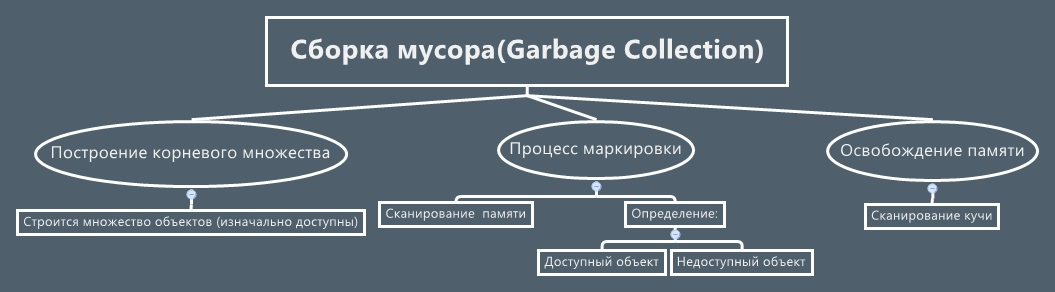
\includegraphics[width=500pt]{picture1}
	\caption{На схеме представлены три основных этапа сборки мусора}
	\centering
\end{figure}

Далее рассмотрим подробнее каждый из этапов в контексте сборщика мусора JBGC,  с которым можно самостоятельно ознакомиться.\footnote{URL: \url{https://github.com/danyaberezun/diploma/tree/master}} Реализация которого описана в \cite{realisation}.



\subsection{Процесс построения корневого множества и объектов кучи}
\subsubsection{Процесс построения корневого множества}
Данный процесс подробно рассмотрен в статье \cite{roots}.
При создании gc\_ptr, стоит учитывать то, что объекты могут создаваться как в куче, так и на стеке. Список стековых объектов  нужно обязательно хранить для того, чтобы уметь в дальнейшем отслеживать состояние объектов, сканировать объекты, начиная с рутов, и помечать мусор. 

Для того, чтобы отслеживать место создания объекта, заведен специальный флаг, который при вызове функции выделения памяти gc\_new  под gc\_ptr декларирует место создания объекта. Если флаг выставлен, значит объект создан в куче, если нет, на стеке.

Все ``умные указатели'' (gc\_ptr), вызывают в своем конструкторе функцию добавления себя в список корней, в случае загрузки стековой рамки на стек и функцию удаления себя из этого списка в своем диструкторе, в случае вытеснения стековой рамки. Статические объектами, являющиеся gc\_ptr, добавляются в список рутов в момент инициализации статической области. Все это происходит внутри класса gc\_ptr.


\subsubsection{Процесс построения метаинформации}
Модель представления объектов для сборки мусора была описана в \cite{meta}. Рассмотрим процесс построения метаинформации.

Когда выделяется память под объект в куче, перед ним кладется указатель на соответствующую ему метаинформацию. Ее нужно конструировать в случае, если при поиске в списке пар (typeid, classMeta), где classMeta -- список указателей на метаинформацию различных типов, не установлено соответствий. Если же поиск успешен, указатель на соответствующую типу метаинформацию вернет функция  поиска.

Процесс построения метаинформации включает в себя создание обертки объекта. Обертка создается в единственном экземпляре для каждого типа, создание происходит в gc\_new. Она хранит в себе смещения указателей вложенных объектов gc\_ptr относительно указателя на объект (это нужно для того, чтобы ходить по всем достижимым объектам). Все смещения записываются внутри функции gc\_new в вектор, а вектор получается из разностей между значением из глобального массива объектов и указателя на начало объекта. 

Основной задачей, решаемой хранением метаинформации, является возможность обхода дерева живых объектов на стадии маркировки, начиная с корней.

\subsection{Процесс маркировки}
При использовании кучи в 64-битной системы, ввиду выравнивания в заголовке объекта, остаётся дополнительный свободный бит, который можно использовать в своих целях. В JBGC он используется для маркировки объекта. Процесс маркировки происходит в функции mark\_and\_sweep(). 
Сначала помечаются ``фейковые руты'', это объекты, которые приравниваются к рутам, и которые пользователь самостоятельно регистрирует или снимает с них регистрацию специальной функцией предоставленной интерфейсом.  ``Фейковые руты'' появляются из-за того, что пользователю  предоставляется возможность совмещения автоматического и ручного управления памятью. В связи с этим появляется проблема: наличие ссылки из ручного на автоматический объект. В случае, если более не осталось ссылок из автоматических объектов на данный объект, а из ручного на него ссылка есть, сборщик мусора удалит рассматриваемый объект, и ссылка станет висящей. Регистрация решает эту проблему.

После маркировки ``фейковых рутов'' происходит рекурсивный обход и маркировка всех объектов, начиная со стековых.

\subsection{Процесс освобождения памяти}

Освобождение памяти происходит внутри функции mark\_and\_sweep(). Вызывается функция sweep(), которая реализована внутри кучи. Функция пробегает по всем элементам кучи,высвобождая память из-под маркированных объектов.
\newpage
\section{Заключение}

Следующие результаты были достигнуты в рамках данной дипломной работы. 

\begin{enumerate}
\item Были изучены и  описаны следующие подходы к неконсервативной и консервативной сборке мусора: [лучше через зпт, а не списком] 1, 2, 3. Также была составлена сравнительная характеристика предоставленных пользовательских уровней для различных языков и сборщиков мусора;

\item На основе проведенного анализа подходов к сборке мусора и сравнительной характеристики, было предложено разработать неконсервативный сборщик мусора для С++ с использованием алгоритма mark\&sweep;
\item Предложенное решение было реализовано на языках С/С++ в рамках проекта JBGC, и были продемонстрированы возможности пользовательского уровня получившегося неконсервативного сборщика мусора;

\item Был проведен сравнительный анализ языковых примитивов языка С++ и набора различных конструкций, предлагаемых к использованию в JBGC;
\end{enumerate}

\vspace{0.3cm}
Данный анализ показал, что текущих наработок достаточно для реализации большинства возможных языковых ситуаций. Но, в конечном счёте, в JBGC всё же существует ряд недоработок и ограничений, с которыми нужно бороться, таких как:
\begin{enumerate}
\item 
\end{enumerate}
%\newpage
\bibliographystyle{plainnat}
\addcontentsline{toc}{section}{Список литературы}
\begin{thebibliography}{}

\bibitem{GCBook} 
Richard Jones, Rafael Lins. Garbage Collection: Algorithms for Automatic Dynamic Memory Management. John Wiley \& Sons, 2001.

\bibitem{roots}
Д.А. Березун. Постоение корневого множества указателей для сборки мусора // Труды лаборатории языковых инструментов JetBrains, 
выпуск 1. Санкт-Петербург, 2013.

\bibitem{meta}
М.В. Крень. Представление данных для сборки мусора // Труды лаборатории языковых инструментов JetBrains, выпуск 1. Санкт-Петербург, 2013.


\bibitem{realisation}
Д.А. Березун. Реализация основных примитивов библиотеки неконсервативной сборки мусора для С++. Дипломная работа, СПбГУ, 2014.


\bibitem{standart}
Bjarne Stroustrup. C++11 --- the new ISO C++ standard // \url{http://www.stroustrup.com/C++11FAQ.html}


\end{thebibliography}

%\newpage
%\include{appendix}

% \bibliographystyle{ugost2008ls}
% \bibliography{diploma.bib}

\end{document}
